\documentclass[12pt]{article}
\usepackage[letterpaper, left=2.5cm, right=2.5cm, top=2.5cm, bottom=2.5cm]{geometry}
\usepackage{float}
\usepackage{subfig}
\usepackage{graphicx} 
\usepackage{array}
\usepackage[utf8]{inputenc}
\usepackage[spanish]{babel}
\decimalpoint
\usepackage{amsmath}
\usepackage{amsfonts}
\usepackage{amssymb}
\usepackage{listings}
\usepackage{makeidx}
\usepackage{hyperref}
\usepackage[dvipsnames]{xcolor}
\definecolor{backcolor}{rgb}{0.95,0.95,1.5} 
\lstdefinestyle{mystyle}{
	backgroundcolor=\color{backcolor},   
	commentstyle=\color{CadetBlue},
	keywordstyle=\color{Plum},
	numberstyle=\tiny\color{Bittersweet},
	stringstyle=\color{Cerulean},
	basicstyle=\ttfamily\footnotesize,
	breaklines=true}
\lstset{style = mystyle}


\title{Tarea 2} 
\author{Ulises Jiménez Guerrero}


\begin{document}
\begin{titlepage}
	\centering
	{\includegraphics[width=0.2\textwidth]{/home/ulisex/Imágenes/logo_UV.png}\par}
	\vspace{1cm}
	{\bfseries\LARGE Universidad Veracruzana \par}
	\vspace{1cm}
	{\scshape\Large Maestría en Inteligencia Artificial \par}
	{\scshape\Large Visión por computadora \par}
	\vspace{3cm}
	{\scshape\Large Tarea 3 \\
		Mejora de imágenes mediante ecualización de histograma\par} 
	\vspace{3cm}
	{\itshape\Large  \par}
	\vfill
	{\Large Ulises Jiménez Guerrero\par}
	\vfill		
	{\Large \today \par}
\end{titlepage} 


\begin{center}
	\Large
		{\scshape Reporte tarea 2}
\end{center}

\section{Objetivos}
\begin{itemize}
	\item Crear un programa de computadora capaz de escalar imágenes, ya sea aumentando o encogiendo su tamaño, utilizando las técnicas de vecino más cercano e interpolación bilineal. La entrada del programa será las dimensiones de la imagen deseada, y su salida las imágenes 
	resultantes con estos métodos.
	
	\item Comprobar el funcionamiento del programa y de cada método utilizando la imagen de prueba proporcionada para ello. 
\end{itemize}
 
 
\section{Metodología}
\subsection{Materiales utilizados}

Para el desarrollo se utilizó el lenguaje de programación Python, versión 3.12.8. Para el manejo de las imágenes se utilizó la paquetería de código libre \href{https://pypi.org/project/opencv-python/}{opencv} para Python, junto a la paquetería \href{https://pypi.org/project/numpy/}{Numpy} para el manejo de las matrices generadas por las imágenes. Finalmente, se utilizó la paquetería de \href{https://pypi.org/project/matplotlib/}{Matplotlib} para el despliegue de imágenes en la pantalla, que a su vez instala varias dependencias. Todas las paqueterías junto a las versiones utilizadas se encuentran listadas en el anexo. Para la comprobación del algoritmo, se utilizó la imagen 2.19 (a) del libro
\cite{gonzalezDigitalImageProcessing2017}
, mostrada en la imagen \ref{fig:rose}. Esta imagen tiene un tamaño original de 
1024$\times$1024 píxeles, y se utilizó en una escala de grises con 8 bits.

\begin{figure}[H]
	\centering
	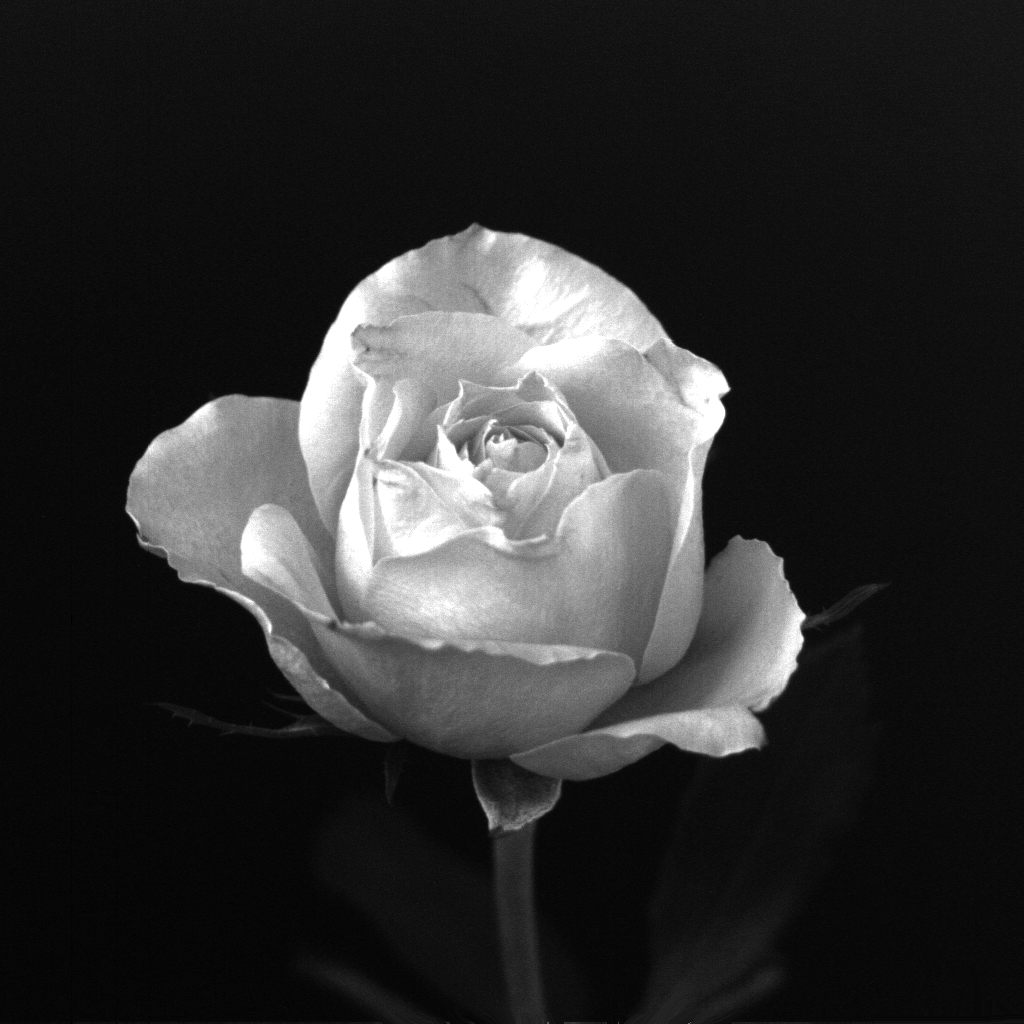
\includegraphics[width=0.5\linewidth]{imgs/rose}
	\caption{Imagen utilizada para probar los algoritmos. Muestra una rosa blanca sobre un fondo negro, con detalles del tallo. No se encuentra a escala.}
	\label{fig:rose}
\end{figure}


\subsection{Algoritmos e implementación}

\subsubsection{Método del vecino más cercano}
Este es el método más sencillo para escalar el tamaño de una imagen digital, y por esto da los peores resultados. Su funcionamiento es sencillo: para cada nuevo píxel de la imagen escalada, se le asigna el valor de la tonalidad del píxel más cercano en la imagen original. Para ello, se debe realizar un mapeo de las coordenadas de la imagen reajustada a la imagen original. Este problema se solventa utilizando la proporción entre las dimensiones de la imagen original y la imagen deseada. De esta forma, un píxel con coordenadas $(i, j)$ en la  imagen ajustada tiene las coordenadas $(x,y)$ en la imagen original, dadas por:

$$
x = i \times r_w, \quad y = j \times r_h 
\quad \text{donde} \quad
r_w = \dfrac{\text{Ancho original}}{\text{Nuevo ancho}}, 
\quad
r_h = \dfrac{\text{Alto original}}{\text{Nuevo alto}}.
$$

Como el cálculo de distancias es un proceso costoso, se realiza una técnica diferente para obtener el píxel más cercano. Se redondea el valor de las coordenadas $(x,y)$ obtenidas y se utiliza la intensidad del píxel $f(x,y)$ con las coordenadas redondeadas. Debido a que existen varios métodos para el redondeo de números, esto puede ocasionar resultados diferentes, pero no a un nivel significativo \cite{wojcickiNearestNeighbourInterpolation2020}. 

Para la implementación realizada se utilizó la función \textit{int()} de Python, que realiza un redondeo hacia abajo. Este es el mismo redondeo utilizado en la función de ajuste de imágenes nativa de opencv  con el método de vecino más cercano. El algoritmo se aplicó de forma directa, generando una matriz vacía con el tamaño indicado por el usuario y aplicando la fórmula  sobre cada píxel, recorriendo la imagen de izquierda a derecha y de arriba a abajo. Cabe destacar que este tipo de ciclos anidados son lentos en Python, donde se recomienda realizar operaciones matriciales en Numpy para mejorar la velocidad de los programas. 

\subsubsection{Método de interpolación bilineal}
Este método es más refinado que el de vecino más cercano, y presenta resultados más suaves y que preservan una mayor calidad de imagen. Sin embargo, esto lo hace más costoso, requiriendo un tiempo de procesado mayor. 

Se empieza con un mapeo de las coordenadas de la nueva imagen a la imagen original, de la misma forma que en el algoritmo anterior. Dada la posición en la imagen original, se obtiene la tonalidad realizando un promedio ponderado en base a los cuatro píxeles más cercanos. Estos se encuentran en la esquina superior derecha, esquina superior izquierda, esquina inferior derecha y esquina inferior izquierda. Para obtener el promedio ponderado se realiza una interpolación tanto en la dimensión $X$ como en la $Y$, esto es, sobre dos líneas, dando su nombre al algoritmo.

 Dado que cada píxel tiene un valor de una unidad de medida, se puede considerar que se trabaja en un cuadrado unitario. Tomando este sistema de referencia, la esquina superior izquierda tiene coordenada $(1,0)$, la inferior derecha $(0,1)$, etc. De esta forma, se tiene la siguiente ecuación para la intensidad del píxel en las coordenadas $(x,y)$, realizando ambas interpolaciones en un solo cálculo:

\begin{multline}
	f(x,y) = \left(f(1,0) - f(0,0) \right)x + \left(f(0,1) - f(0,0)\right)y
	\\
	+ \left( f(1,1) - f(0,0) - f(0,1) - f(1,0) \right)xy + f(0,0)
	\label{eq1}
\end{multline}

La implementación se realizó de forma directa, generando una matriz vacía con las dimensiones adecuadas y recorriendo cada píxel, calculando su intensidad mediante el método indicado. Se realizaron algunas modificaciones a \ref{eq1}, sugeridas en \cite{wojcickiBilinearInterpolation2022}
para simplificar cálculos. Sin embargo, sigue siendo una operación costosa, tomando varios segundos para procesar imágenes de tamaños mayores a $1000\times1000$ píxeles. Para la obtención de los píxeles vecinos más cercanos, se utilizó la función \textit{floor()} de numpy para obtener un redondeo hacia abajo, dando los valores inferiores en los ejes X y Y. Para los valores superiores, se sumo 1 a estos resultados. Sin embargo, se debe prestar especial atención a los píxeles ubicados en los bordes de la imagen. Existen diversas técnicas para lidiar con ellos, como realizar una copia del borde alrededor de la imagen. En nuestro caso, se utilizó la función \textit{min()} para asegurarnos que la coordenada obtenida siempre se mantiene dentro de los límites de la imagen, aunque esto resulte en que se repita el mismo píxel en algunos cálculos. 

\subsubsection{Manejo de las imágenes}
Con el uso de la función \textit{imread()} de opencv, se leyeron a las imágenes como matrices de numpy, fáciles de manipular en Python. Se estableció el canal de color como escala de grises, de manera que se utilizaron matrices de tamaño $(\text{Pixeles de ancho} \times \text{Pixeles de alto})$, donde el valor de cada celda se corresponde a la intensidad de la tonalidad de gris en ese píxel. Las matrices resultantes de los algoritmos se guardaron como imágenes formato PNG, lo que facilita su inclusión en el reporte. Además, con el uso de matplotlib se implementó la opción de visualizar las imágenes resultantes junto a la imagen original, ajustando el tamaño del píxel para que ocupen el mismo espacio en la pantalla, lo que permitió una mejor comparación de la calidad de imagen resultante. 

\section{Resultados}
Se inició contrayendo la imagen en \ref{fig:rose} a un tamaño de 
$256 \times 256$ píxeles, esto es, un cuarto de su tamaño. Las imágenes resultantes se pueden observar en \ref{img:compresion_rose}. La pérdida de calidad en la imagen es evidente para ambos métodos, sobre todo en los bordes de los pétalos de la rosa. No se observa una diferencia en los resultados de los dos métodos, debido a que la pérdida de información es significativa en ambos casos.

\begin{figure}[htbp]
	\centering
	\subfloat[Compresión de imagen mediante vecino más cercano. Escala real,]{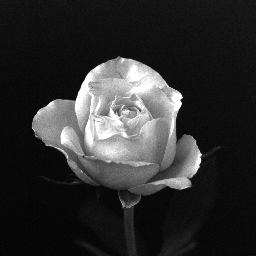
\includegraphics[scale=1]{imgs/shrinked_img_nn.png}}
	\quad
	\subfloat[Compresión de la imagen mediante interpolación bilineal. Escala real.]{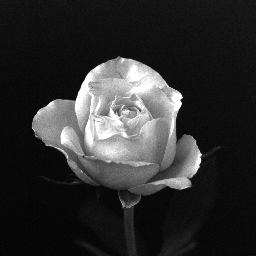
\includegraphics[scale=1]{imgs/shrinked_img_bi.png}}
	\caption{Resultados de la compresión de la imagen de prueba.}
	\label{img:compresion_rose}
\end{figure}

\clearpage

Posteriormente, se tomó cada una de las dos imágenes resultantes y se aplicaron ambos métodos para re-escalarlas a su tamaño original de 
$1024\times1024$ píxeles. Los resultados se muestran en las figuras 
\ref{img:expansion_rose_nn} y \ref{img:expansion_rose_bi}. Ninguna de las cuatro imágenes presenta una calidad igual a la original. Esto es de esperarse, dado que el proceso de interpolación siempre pierde información y agrega ruido a la imagen, efecto que se va sumando mientras más veces se realice este proceso sobre la misma imagen. De todas las imágenes obtenidas, la que tiene un resultado más suave es aquella que se sometió al proceso de interpolación bilineal dos veces, una para compresión y otra para expansión. Aunque en una revisión rápida pueda parecer que su calidad no difiere significativamente de \ref{fig:rose}, una revisión más detallada muestra la presencia de ruido en los bordes del pétalo, además de una pérdida de la suavidad de su forma y un cambio más brusco en la tonalidad. Métodos más sofisticados como interpolación bicúbica permiten realizar este proceso de forma más eficaz, pero la pérdida de información inherente a los métodos de interpolación no se logra eliminar. 

 \begin{figure}[htbp]
 	\centering
 	\subfloat[Expansión de la imagen mediante vecino más cercano.]{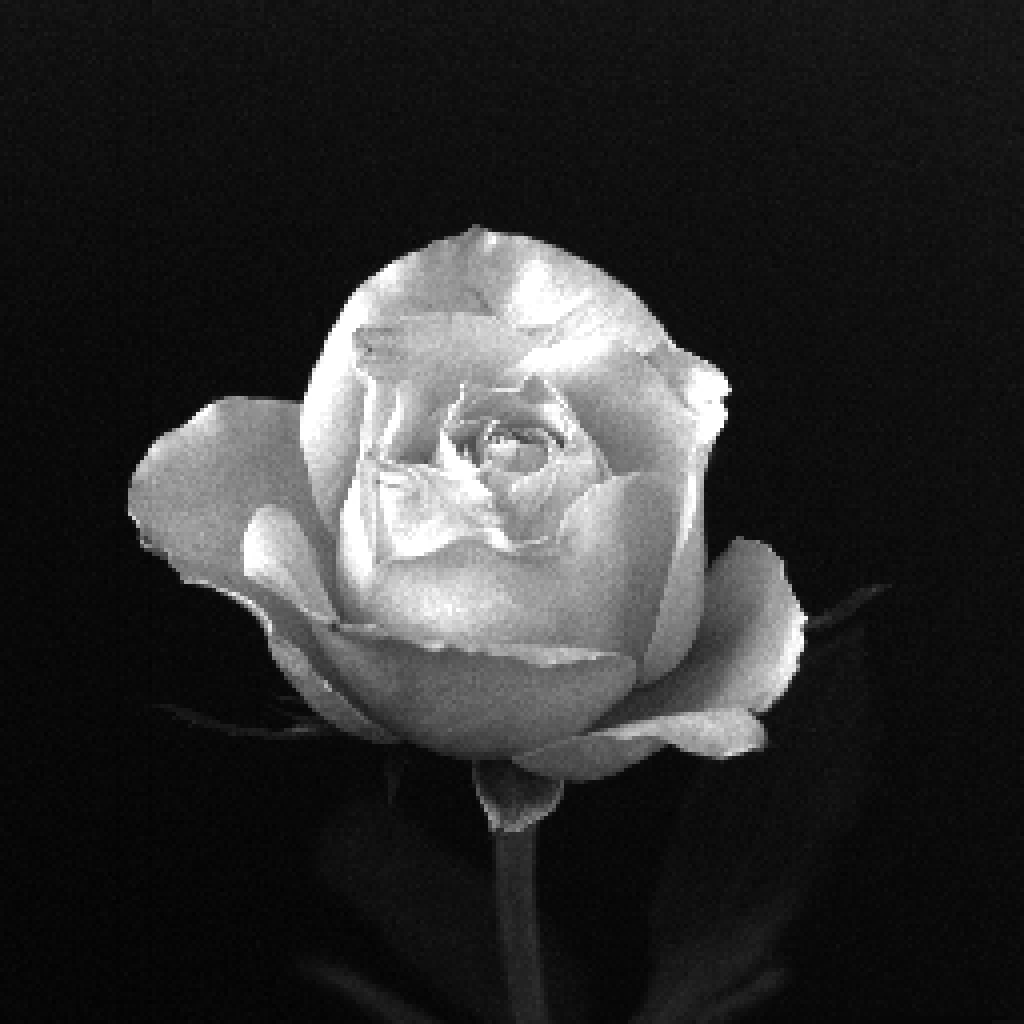
\includegraphics[width=0.5\textwidth]{imgs/expanded_img_nn2nn.png}}
 	\quad
 	\subfloat[Expansión de la imagen mediante interpolación bilineal.]{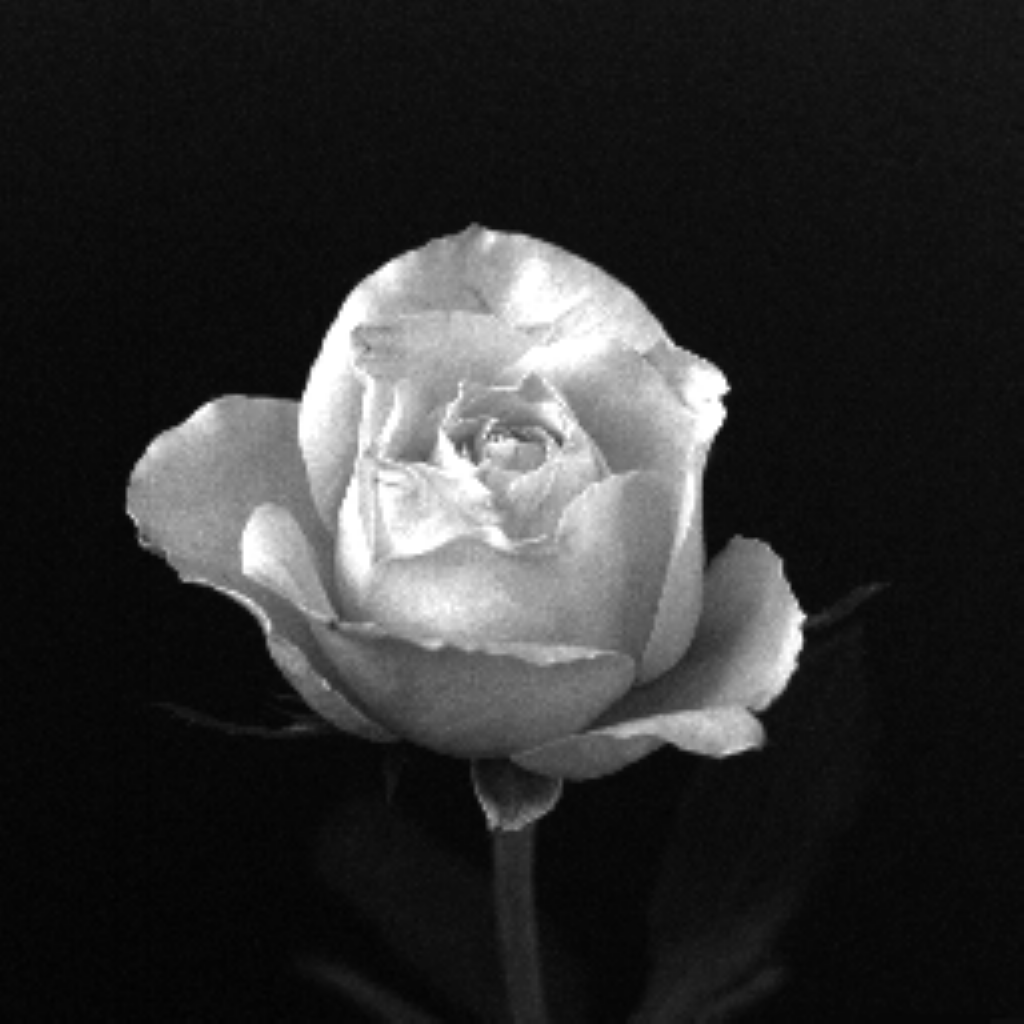
\includegraphics[width=0.5\textwidth]{imgs/expanded_img_nn2bi.png}}
 	\caption{Resultados de la expansión de la imagen comprimida obtenida mediante el método del vecino más cercano.}
 	\label{img:expansion_rose_nn}
 \end{figure}


\begin{figure}[htbp]
	\centering
	\subfloat[Expansión de la imagen mediante vecino más cercano.]{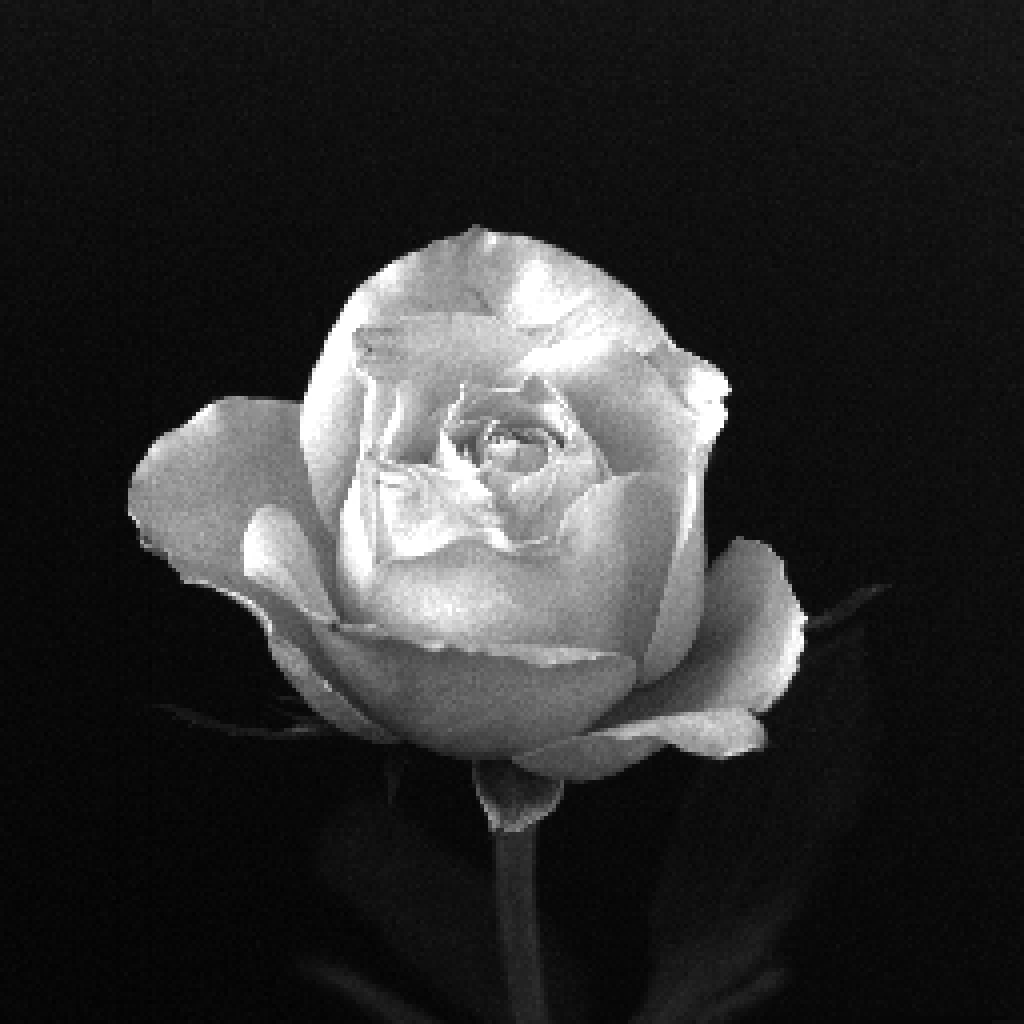
\includegraphics[width=0.5\textwidth]{imgs/expanded_img_bi2nn.png}}
	\quad
	\subfloat[Expansión de la imagen mediante interpolación bilineal. ]{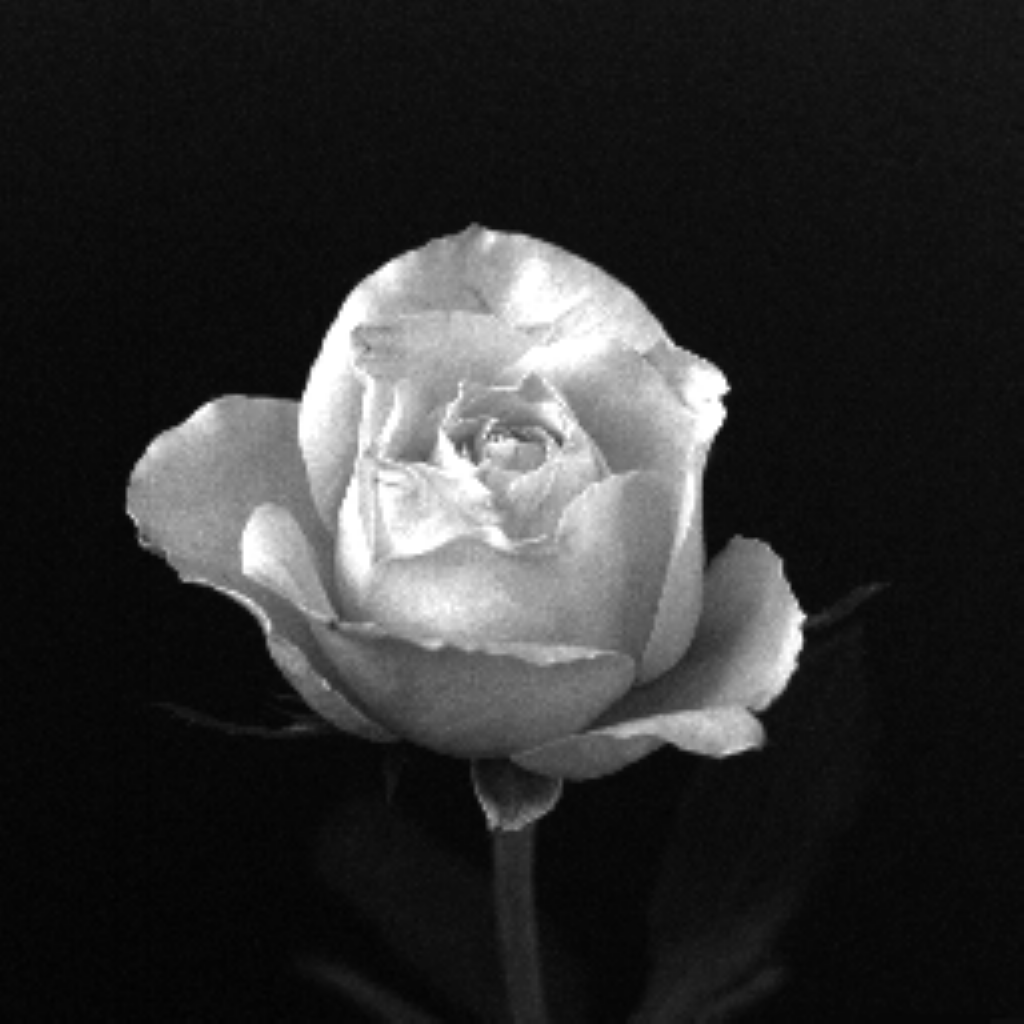
\includegraphics[width=0.5\textwidth]{imgs/expanded_img_bi2bi.png}}
	\caption{Resultados de la expansión de la imagen comprimida obtenida mediante el método de interpolación bilineal.}
	\label{img:expansion_rose_bi}
\end{figure}

\section{Conclusiones}
El método de interpolación mediante vecino más cercano es sencillo de implementar y de calcular, lo que lo hace ideal para situaciones donde se busca un ajuste mínimo de las dimensiones de una imagen. Para estos casos, la pérdida de información es despreciable, y su uso es adecuado. En cambio, cuando el cambio en el tamaño de la imagen original es significativo, se requieren de métodos más sofisticados como la interpolación bilineal para mantener la calidad de imagen original lo más posible. Sin embargo, para cambios extremos como el realizado en este trabajo, este método sigue presentando defectos notables a simple vista, lo que indica que se requieren técnicas todavía más avanzadas como la interpolación bicúbica. Un trabajo a futuro sería el comparar el desempeño de este algoritmo con los ya implementados.

Algo que destacó este trabajo es que se debe evitar redimensionar la misma imagen múltiples veces, dado que el efecto de la pérdida de información se suma en cada iteración, y la calidad de la imagen decae rápidamente. En casos donde se requiera la misma imagen en diferentes resoluciones, siempre se debe aplicar la transformación sobre la imagen original, minimizando de esta manera la pérdida de calidad. 

\bibliographystyle{plain}
\bibliography{tarea2_fuentes.bib}

\section{Anexo}
\subsection{Lista de paqueterías y versiones}
\begin{itemize}
	\item contourpy==1.3.1
	\item cycler==0.12.1
	\item fonttools==4.56.0
	\item kiwisolver==1.4.8
	\item matplotlib==3.10.0
	\item numpy==2.2.3
	\item opencv-python==4.11.0.86
	\item packaging==24.2
	\item pillow==11.1.0
	\item pyparsing==3.2.1
	\item python-dateutil==2.9.0.post0
	\item six==1.17.0
\end{itemize}

\subsection{Código}
\lstinputlisting[language=Python]{img_resize.py}

\end{document}